%!TEX root = ../main.tex
\vspace*{\fill}

{\large \bf Chapter~\ref{chp:sln_orth_pdf} Authorship Statement}

\vspace{1em}

{\bf Citation:} S{\o}ren Asmussen, Pierre-Olivier Goffard, Patrick J.\ Laub (2015), \emph{Orthonormal polynomial expansions and lognormal sum densities}, Risk and Stochastics: Ragnar Norberg at 70 (Mathematical Finance Economics), World Scientific

\vspace{1em}

The authors of this paper equally contributed to the following tasks:
\begin{enumerate}
\item conception and design of the project;
\item mathematical arguments, and interpretation of the results;
\item writing the publication.
\end{enumerate}

In addition to this, I completed the majority of the computational work and of the editing (e.g.\ checking grammar and typographical details).

\vspace{3em}

\vspace*{\fill}

\chapter{Orthonormal polynomial expansions and densities of sums of lognormals} \label{chp:sln_orth_pdf}

\section{Introduction}\label{S:SLN_Ortho_PDF_Intr}

The previous chapter considered approximating the SLN Laplace transform and used this to approximate distribution's pdf. This chapter discusses a different method where one approximates the SLN pdf $f$ using polynomials $\{p_k\}_{k\in\NZ}$ which are orthonormal w.r.t.\ some reference pdf $w$. In the general formulation, one is interested in approximating a target density $g$ using the pdf $w$ as reference.
One then finds
a series representation of $g/w$ of the form $\sum_{k=0}^\infty a_k p_k$,
and then the approximation of $g$ is
\begin{equation} \label{orthog_approx}
	\widehat{g}(x)\ =\ w(x) \sum_{k=0}^K a_k p_k(x),
\end{equation}
for some suitable $K$.
The most obvious connection to the sum of lognormals problem is $g=f$, but for some choices of $w$ we must take a different target $g$. In one case we set $g$ as the density of $\log S$ and transform back to get the approximation $\widehat{f}(x)=$
$\widehat{g}(\log x)/x$. In another case we set $g$ as the exponentially tilted SLN pdf.
The choice of $w$ is a crucial step, and three candidates for $w$ are investigated, the pdfs of the normal, gamma, and lognormal distributions.

The form of the $p_k$ is classical for the normal distribution where it is the Hermite polynomials and for the gamma where  it is the generalised Laguerre polynomials,
but for the lognormal distributions it does not appear to be in the literature and we give here  the functional expression
(\thrm{LogNormalOrthogonalPolynomialProposition}). The Fenton--Wilkinson method may be seen
as the $K=2$ case of $w$ being lognormal (with $g=f$), and this choice of $w$  may be the most obvious one.
However, we show that in the lognormal case the orthonormal polynomials are not dense in $\Lp^2(\RL, w(x) \dd x)$. This result is closely related
to the lognormal distribution not being determined by its moments
\cite{Heyde63,Berg1984} and indicates that a lognormal $w$ is potentially dangerous.
For this reason, the rest of the chapter concentrates on  taking the reference distribution as normal (using the logarithmic transformation)
or gamma  (using exponential tilting).

Applying orthogonal polynomial expansions to sums of lognormals is not a new idea; many papers, whose motivation relates to pricing Asian options, have contributed to this task. The earliest relevant work on this is from Turnbull and Wakeman \cite{turnbull1991quick}, who constructed an orthogonal polynomial expansion for the sum of correlated lognormals using a lognormal reference distribution. Dufresne and Li refer state of this: ``the convergence of those \dots series has never been proved, and their theoretical convergence is highly unlikely'' \cite[p.\ 1]{dufresne2016pricing}. This conjecture is precisely what we have proved here, showing the incompleteness of the lognormal orthogonal polynomials in $\Lp^2(\RL, w(x) \dd x)$.

The next development was Dufresne \cite{dufresne2000laguerre} who tackled the related problem of pricing continuous Asian options --- here the underlying average is $A = \frac1T \int_0^T \e^{X_t} \dd t$ where $\{X_t\}_{t\in[0,T]}$ is a Brownian motion. They use an orthogonal polynomial expansion using a gamma reference distribution, and sidestep the integrability problem by approximation the pdf of $1/A$ rather than $A$. The expansion's coefficient are constructed from the moments of $1/A$, which are found using a recursive scheme of symbolic integrations in \textsc{Mathematica}.

Popovic and Goldsman \cite{popovic2012easy} consider the problem pricing discrete Asian options --- that is, the underlying average is $A = \frac1n \sum_{i=1}^n \e^{X_i}$ where $\{X_i\}_{i\in\NZ}$ is a discretely observed Brownian motion (they consider stock prices driven by other L{\'e}vy processes, e.g., the variance-gamma process). They construct an orthogonal expansion of $\log(A)$ using a normal reference distribution, and evaluate the coefficients using Monte Carlo (with some variance reduction techniques). Dufresne and Li \cite{dufresne2016pricing} take the same approach, but add in the theory which was missing by giving the conditions so that the orthogonal expansion will converge. They also write the explicit form of an Asian option price given this orthogonal polynomial approximation for $\log(A)$. Lastly, the paper from Chateau and Dufresne \cite{chateau2017gram}, which is more recent than the contents of this chapter, ought to be noted to complete this review.

As noted above, we are the first to derive the orthogonal polynomials w.r.t.\ the lognormal reference, and prove their incompleteness in the relevant space. Our normal reference approximation is applied to the logarithm of the sum, akin to \cite{popovic2012easy} and \cite{dufresne2016pricing}. The gamma reference approximation is not applied to the reciprocal random variable, like \cite{dufresne2000laguerre}, but to the exponentially tilted sum of lognormal distribution.

After discussing the details of the orthonormal polynomials expansions in Sections~\ref{S:OrthPol} and~\ref{S:LN_Appl},
we proceed in Section~\ref{S:numerical} to show a number of numerical examples. The polynomial expansions
are compared to existing methods as Fenton--Wilkinson and a more recent approximation in terms of log skew normal
distributions \cite{hcine2015highly}, as well as to exact values obtained by numerical quadrature in cases where this
is possible or by Monte Carlo density estimation. Section~\ref{S:numerical} also outlines an extension to  statistical data sets and non-Gaussian copulas. Appendix A contains a technical proof
and Appendix B some new material on the SLN Laplace transform.

\section{Orthogonal polynomial representation of probability density functions}
\label{S:OrthPol}

Let $X$ be a random variable which has a density $f$. If $f$ is unknown but the distribution of $X$ is
expected to be close to some pdf $w$, one may use $w$ as a first approximation to $f$ and next try
to improve by invoking suitable correction terms.

In the setting of this chapter $X$ is the sum of lognormal random variables and the correction terms are obtained by expansions in terms of orthonormal polynomials.
Before going into the details of the lognormal example, let us consider the general case.

Assuming all moments of $w$ to be finite,
the standard Gram--Schmidt orthogonalisation technique shows the existence
of a set of polynomials $\{p_k\}_{k\in\NZ}$ which are orthonormal in
$\Lp^2(\RL, w(x) \dd x)$ equipped with the usual inner product
$\langle g, h \rangle_w$ and the corresponding norm
$\norm{g}^2$.
From Proposition~\ref{prop:complete_polynomials}, we know that if there is an $\alpha>0$ such that
\begin{equation}\label{DefinedMGFCondition}
\int_{\RL} \e^{\alpha|x|} w(x) \dd x < \infty\,,
\end{equation}
then the polynomials $\{p_k\}_{k\in\NZ}$ are complete in $\Lp^2(\RL, w(x) \dd x)$. The implication is that if $f/w \in \Lp^2(\RL, w(x) \dd x)$, that is, if
\begin{equation}\label{L2Condition1}
\int_{\RL} \frac{f(x)^2}{w(x)^2} w(x) \dd x\ =\ \int_{\RL} \frac{f(x)^2}{w(x)} \dd x\ <\ \infty\,,
\end{equation}
we may expand $f/w$ as $\sum_{k=0}^\infty a_k p_k$ where
\begin{align}\label{28.10a}a_k\ &=
\langle f/w, p_k \rangle_w\ =\ \int_{\RL} f(x) p_k(x) \dd x\ =\ \Exp\left[p_k(X)\right]\,.
\end{align}
This suggests that we use the form of \eqref{orthog_approx} as an approximation of $f$ in situations where the pdf of $X$ is unknown but the moments are accessible.

\begin{remark}\label{Rem:27.10a}
If the first $m$ moments of $X$ and $w$ coincide, one has $a_k=0$ for $k=1$, \ldots, $m$, which is a consequence of the linear independence of the orthogonal polynomials.
When choosing $w$, a possible guideline is therefore to match as many moments as possible.
\remQED
\end{remark}

Due to the Parseval relationship $\sum_{k=0}^\infty a_k^2=\norm{f/w}^2$, the coefficients of the polynomial expansion, $\{a_k\}_{k\in\NZ}$, tend toward $0$ as $k \to \infty$.
The accuracy of the approximation \eqref{orthog_approx}, for a given order of truncation $K$, depends upon how swiftly the coefficients decay; note that the $\Lp^2(\RL, w(x) \dd x)$ loss of the approximation of $f/w$ is $\sum_{K+1}^{\infty}a_k^2$.
Note also that the orthogonal polynomials can be specified recursively
(see Thm.~3.2.1 of \cite{Szegoe1939}) which allows a reduction of the computing time required for the coefficients' evaluation
and makes it feasible to consider rather large $K$.

\subsection{Normal reference distribution}\label{SS:NormalNu}
A common choice as a reference distribution is the normal $\NormDist(\mu,\sigma^{2})$. The associated orthonormal polynomials are given by
\begin{equation}\label{eq:NormalDistributionOrthogonalPolynomial}
p_{k}(x)=\frac{1}{k!2^{k/2}}H_{k}\left(\frac{x-\mu}{\sigma\sqrt{2}}\right),
\end{equation}
where $\left\{H_{k}\right\}_{k\in\NZ}$ are the (physicists') Hermite polynomials, defined in \cite{Szegoe1939} for instance.
If $f$ is continuous, a sufficient (and close to necessary) condition for $f/w\in\Lp^2(\RL, w(x) \dd x)$ is
\begin{equation}\label{SA7.11a}
f(x)\ =\ \Oh(\e^{-ax^2})\quad\text{as }x\to\pm\infty\quad\text{with } a>(4\sigma^2)^{-1}\,.
\end{equation}
Indeed, we can  write the integral in \eqref{L2Condition1} as $I_1+I_2+I_3$, the integrals over
$(-\infty,-A)$, $[-A,A]$, resp.\ $(A,\infty)$. Note that $I_2<\infty$  follows since the integrand
is finite by continuity, whereas the finiteness of $I_1,I_3$ is ensured by the integrands
being $\Oh(\e^{-bx^2})$ where $b=2a-1/2\sigma^2>0$. Similar arguments apply to
conditions \eqref{SA7.11b} and \eqref{SA7.11c} below.

\begin{example}\label{Ex:27.10a}
The classical example of this technique (though not usually put in this framework)
is the \emph{Edgeworth expansion}, which is almost identical to the \emph{Gram--Charlier expansion of type A}.
Consider $Y_1$, \dots $Y_n$ iid random variables where $\Exp[Y_i]=\mu$ and $\Var[Y_i]=\omega^2$.
The Edgeworth expansion covers $X=(S-n\mu)/(\sqrt{n}\,\omega)$ with the $\NormDist(0,1)$ density as the reference pdf.

The Edgeworth example illustrates well several aspects of the theory. In the scenario of Remark~\ref{Rem:27.10a} with $m=2$, condition~\eqref{DefinedMGFCondition} is trivially satisfied,
but condition~\eqref{L2Condition1} requires more attention. It actually fails unless
$f(x)$ decays very quickly as $x \to\pm \infty$, even in such a basic example as the $Y_i$
being standard exponential (then $f(x)$ is of order $x^{n-1} \e^{-xn^{1/2}}$
which multiplied by $\e^{x^2/2}$ does not integrate). Nevertheless, the Edgeworth approach
has been observed to perform well even when condition~\eqref{L2Condition1} is not satisfied;
in fact, the condition is only sufficient, not necessary (Cram{\'e}r \cite{cramer1926some} showed it can be relaxed to
$\Exp [\e^{X^2/4}]<\infty$).
\remQED
\end{example}

\subsection{Gamma reference distribution}\label{SS:GammaNu}
If $X$ has support $(0,\infty)$, it is natural to look for a $w$ with the same property.
An obvious candidate is the gamma distribution, denoted $\GammaDist(r,m)$ where $r$ is the shape parameter
and $m$ the scale parameter. The pdf is
\begin{equation} \label{GammaPDF}
w(x)=\frac{x^{r-1} \e^{-x/m}}{m^{r}\Gamma(r)},\hspace{0.2cm}x\in \RL_+ \,.
\end{equation}
The associated polynomials are given by
\begin{equation} \label{OrthogonalPolynomialGammaDistribution}
p_{n}(x)=(-1)^{n}\left[\frac{\Gamma(n+r)}{\Gamma(n+1)\Gamma(r)}\right]^{-1/2}L_{n}^{r-1}(x/m),\hspace{0.2cm} n\in\NZ,
\end{equation}
where $\{L^{r-1}_{n}\}_{n\in\NZ}$ denote the \emph{generalised Laguerre polynomials}, see \cite{Szegoe1939}; in \textsc{Mathematica} these are accessible via the \texttt{LaguerreL} function.
The polynomials defined in \eqref{OrthogonalPolynomialGammaDistribution} satisfy the recurrence relationship
\begin{eqnarray} \label{OrthogonalPolynomialGammaDistributionRecurreceRelationship}
np_{n}(x)&=&\left(\frac{x}{m}-2n-r+2\right)p_{n-1}(x)\sqrt{\frac{n}{n+r-1}}\nonumber\\
&-&(n+r-2)p_{n-2}(x)\sqrt{\frac{n(n-1)}{(n+r-1)(n+r-2)}}.
\end{eqnarray}
The recurrence relationship will be employed later to speed up the computation of the coefficients.
A sufficient condition, similar to \eqref{SA7.11a}, for $f/w\in\Lp^2(\RL, w(x) \dd x)$ is:
\begin{equation} \label{SA7.11b}
\begin{alignedat}{4}
f(x)\ &=\ \Oh(\e^{ -\delta x }) \quad &&\text{as } x\to\infty \quad && \text{with } \delta>1/2m\,, \text{ and }\\
f(x)\ &=\ \Oh(x^\beta) \quad &&\text{as } x\to 0 \quad && \text{with } \beta>r/2-1\,.
\end{alignedat}
\end{equation}

\subsection{Lognormal reference distribution}\label{SS:LogNNu}
We denote the lognormal distribution as $\e^Y \sim \LNDist(\mu, \sigma^2)$ where $Y \sim \NormDist(\mu, \sigma^2)$. It has support on $\RL_+$. The polynomials orthogonal to the lognormal distribution are given in the following proposition, to be proved in the Appendix:

\begin{theorem}\label{LogNormalOrthogonalPolynomialProposition}
The polynomials orthonormal w.r.t.\ the $\LNDist(\mu, \sigma^2)$ pdf are
\begin{equation}\label{eq:OrthonormalPolynomialLogNormalExpression}
p_{k}(x) = \frac{ \e^{-\frac{k^{2}\sigma^{2}}{2}} }{ \sqrt{[\e^{-\sigma^{2}} ; \e^{-\sigma^{2}}]_k} } \sum_{i=0}^{k}(-1)^{k+i}\e^{-i\mu-\frac{i^{2}\sigma^{2}}{2}}e_{k-i}(1,\ldots,\e^{(k-1)\sigma^{2}})x^{i},
\end{equation}
for $k\in\NZ$ where the $e_i$ are the elementary symmetric polynomials
\begin{equation}\label{eq:ElementarySymmetricPolynomial}
e_i(x_{1},\ldots,x_{k}) =
\begin{cases}
1 &\mbox{for } i = 0, \\
\sum_{1\leq j_{1}<\ldots<j_{i}\leq k}x_{j_{1}}\ldots x_{j_{i}}, &\mbox{for } 1 \leq i\leq k, \\
0,& \mbox{for } i>k,
\end{cases}
\end{equation}
and $[x; q]_{n}=\prod_{i=0}^{n-1}\left(1-xq^{i}\right)$ is the $q$-Pochhammer symbol.
\end{theorem}

\begin{remark}\label{Rem:27.10b}
The result of \thrm{LogNormalOrthogonalPolynomialProposition}
does not appear to be in the literature; the closest reference
seems to be a 1923 paper by Wigert~\cite{Wi23} who considers
the distribution with pdf
$\ell\e^{-\ell^{2}\ln^{2}(x)}/\sqrt{\pi}$, for $x>0$, introduced by Stieljes \cite[pp.\ 507--508]{St1894} (later called the Stieltjes--Wigert distribution). These polynomials are also mentioned in \cite[pp.\ 172--175]{Ch11}.
\remQED \end{remark}

The equivalent of condition \eqref{SA7.11a} for $f/w\in\Lp^2(\RL, w(x) \dd x)$ now becomes
\begin{align}\label{SA7.11c}
f(x)\ &=\ \Oh(\e^{ -b \log^2x } )\quad\text{for }x\to 0 \text{ and } \infty \quad\text{with } b> (4\sigma^2)^{-1}\,,
\end{align}
which is rather mild. However,
a key difficulty in taking the reference distribution as lognormal is the following
result related to the fact that the lognormal and the Stieltjes--Wigert distributions are not characterised by their moments, see \cite{Heyde63,Berg1984,Ch79,Ch03}. Hence, the orthogonal polynomials associated with the lognormal pdf and the Stieltjes--Wigert pdf are also the orthogonal polynomials for some other distribution.
\begin{proposition} \label{prop:ln_incomplete} The set of orthonormal polynomials in
\thrm{LogNormalOrthogonalPolynomialProposition} is incomplete
in $\Lp^2(\RL, w(x) \dd x)$. That is, {\rm span}$\{p_k\}_{k \in \NZ}$ is a proper subset of $\Lp^2(\RL, w(x) \dd x)$.
\end{proposition}
\begin{proof} Let $Y$ be a random variable whose distribution is the lognormal with pdf $w(x)$
and $X$ a random variable with a distribution different from $Y$
but with the same moments. According to \cite[pp.\ 201--202]{Berg1984} such an $X$ can be
chosen such that $f_X/w$ is bounded and hence in $\Lp^2(\RL, w(x) \dd x)$. The projection of
$f_X/w$  onto ${\rm span}\{p_k\}$ is then
\begin{align*}\sum_{k=0}^\infty \langle f_X/w, p_k \rangle_w \, p_k\ &=\
\sum_{k=0}^\infty \Exp\left[p_k(X)\right]p_k\ =\ \sum_{k=0}^\infty \Exp\left[p_k(Y) p_0(Y) \right]p_k\\
&=\ p_0\ =\ 1\,\neq f_X/w,
\end{align*}
where the first step used \eqref{28.10a}, the second step that the moments are the same (and that $p_0 \equiv 1$), and the third follows by orthogonality of the polynomials.
This implies $f_X/w\in\Lp^2(\RL, w(x) \dd x)\setminus{\rm span}\{p_k\}$ and the assertion.
\end{proof}

\subsection{Convergence of the estimators  w.r.t.\ $K$ }

Orthogonal polynomial approximations generally become more accurate as the order of the approximation $K$ increases. \fig{fig:converg} shows a specific orthogonal polynomial approximation, $\widehat{f}_{\mathrm{N}}$ (which involves a logarithmic transformation and is described in Section~\ref{SS:LNNormalNu}), converging to the true SLN density $f$ for increasing $K$. In this example, we take the SLN distribution with $\mu=(0,0,0)^\tr$, $\Sigma_{ii} = 0.1$, and $\rho = -0.1$.

\begin{figure}
\centering
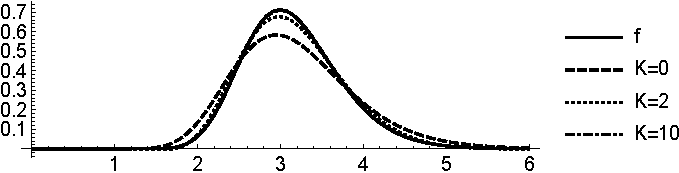
\includegraphics[width=0.8\textwidth]{convergence.pdf}
\caption{Examples of orthogonal polynomial approximations using a $\NormDist(1.13,0.23^2)$ reference converging to the target $f$ with increasing $K$.}
\label{fig:converg}
\end{figure}

\prop{prop:ln_incomplete} implies that orthogonal polynomial approximations with a lognormal reference distribution cannot be relied upon to converge to the desired target density but may have a different limit (the orthogonal projection described there). The next plot, \fig{fig:bad_converge}, illustrates this phenomenon. The approximation appears to converge, but not to the target density.
Our theoretical discussion suggests that this incorrect limit density has the same moments as the target lognormal distribution,
and this was verified numerically for the first few moments.

\begin{figure}
\centering
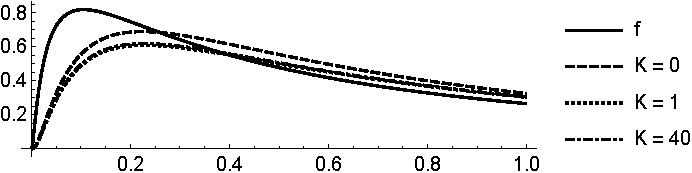
\includegraphics[width=0.8\textwidth]{invalid_convergence.pdf}

\caption{Example of orthogonal polynomial approximations of $f$ using a $\LNDist(0, 1.22^2)$ reference not converging to the $\LNDist(0, 1.50^2)$ target.}
\label{fig:bad_converge}
\end{figure}

Lastly, it must be noted that we cannot in practice take $K$ arbitrarily large, due to numerical errors incurred in calculating the $\{a_k\}$ coefficients. Obviously this can be overcome by using infinite precision operations, however this swiftly becomes prohibitively slow. Software tools like \textsc{Mathematica} allow for arbitrarily large but finite precision, which gives on the flexibility to choose a desired accuracy/speed trade-off. We use this technology and select $K \le 40$.

\section{Application to sums of lognormals} \label{S:LN_Appl}
Now we turn to our main case of interest where $X=S$ is a sum of lognormals. Specifically,
\begin{equation}\label{7.12a}
S=\e^{X_1}+\ldots+\e^{X_n} \,,\quad n \ge 2\,,
\end{equation}
where the vector $\bfX=(X_1,\ldots,X_n)$ is governed by a multivariate normal distribution $\NormDist(\bfmu, \bfSigma)$, where $\bfmu=(\mu_{1},\ldots,\mu_{n})^\tr$ is the mean vector and $\bfSigma=(\sigma_{ij})$ the covariance matrix.
This distribution is denoted $\SLNDist(\bfmu, \bfSigma)$, and hereafter $f$ will be its pdf. We are interested in computing the pdf when the summands exhibit dependency ($\bfSigma$ is non-diagonal). This is an ambitious goal given that the pdf of the sum of two iid lognormally distributed random variables is already unknown. The validity of the polynomial approximations rely on the $\Lp^2$ integrability condition~\eqref{L2Condition1}, which is difficult to check because the pdf of $S$ is not available. This challenge is solved by using asymptotic results describing the left and the right tail of the distribution of $S$, which are collected in the following subsection.

\subsection{Tail asymptotics of sums of lognormals}\label{SS:LNSumsAsympt}

The tail asymptotics of $f(x)$ are given in the following lemma, which simply collects the results from Corollary~2 of \cite{tankov2015tail} and Theorem~1 of \cite{asmussen2008asymptotics}.

\begin{lemma} \label{le:SLNTails}
We have
\begin{eqnarray}
	f(x) &=&  \Oh ( \e^{-c_1 \ln(x)^2} ) \text{ as }x\to 0 \text{ and } \label{SLNLeftTail} \\
	f(x) &=& \Oh ( \e^{-c_2 \ln(x)^2} ) \text{ as }x\to \infty \label{SLNRightTail}
\end{eqnarray}
where
\[
	c_1 = \bigl[ 2 \min_{\bm{w} \in \Delta} \bm{w}^\tr \bm{\Sigma} \bm{w} \bigr]^{-1} \, \text{ and } \,\,\, c_2 = \bigl[ 2 \max_{i=1,\dots,n} \sigma_{ii} \bigr]^{-1}  \,,
\]
with the notation that $\Delta = \{ \bm{w} \,|\, w_i \in \RL_+, \sum_{i=1}^n w_i = 1 \}$.
\end{lemma}

We are also interested in the asymptotic behaviour of $Z = \ln(S)$ later in the chapter. L'H\^opital's rule gives us the asymptotic tails (extending \cite{gao2009asymptotic}) of $f_Z(z) = \e^{z}f(\e^{z})$ to be:

\begin{corollary} \label{co:LogSLNTails}
We have
\begin{align} \label{LogSLNLeftTail}
	f_Z(z)  \ &=\  \Oh(\e^{-c_1 z^2} ) \text{\ as } z\to -\infty
	 \text{ and } \\
 \label{LogSLNRightTail}
	f_Z(z) \ &=\ \Oh(\e^{-c_2 z^2}) \text{\ as } z \to +\infty
\end{align}
where the constants are as in Lemma~\ref{le:SLNTails}.
\end{corollary}

\subsection{Sums of lognormals with a normal reference distribution} \label{SS:LNNormalNu}

Consider transforming the sum to $Z=\ln(S)$ and expanding this density with orthogonal polynomials using a normal distribution as reference. That is, our approximation to $f$ using a $\NormDist(\mu, \sigma^2)$ reference is
\[ \widehat{f}_{\mathrm{N}}(x) = \frac{1}{x} \widehat{f}_{Z}\left(\ln x \right) \quad\text{where}\quad \widehat{f}_{Z}(z) = \phi_{\mu,\sigma^2}(z) \sum_{i=1}^K a_i \, p_i(z) \,, \]
with  the normal pdf $\phi_{\mu,\sigma^2}=w$. The following result tells us when the integrability condition $f_{Z}/w \in\Lp^2(\RL, w(x) \dd x)$ is satisfied.


\begin{proposition}\label{eq:IntegrabilityConditionNormalHermiteExpansion}
Consider $Z=\ln(S)$ where $S \sim \SLNDist(\bfmu,\bfSigma)$. Let $w$ be the pdf of the $\NormDist(\mu,\sigma^2)$ distribution. We have $f_Z / w \in\Lp^2(\RL, w(x) \dd x)$ if
\begin{equation} \label{normal_int_cond_1}
	2 \sigma^2 > (2 c_2)^{-1} = \max_{i=1,\dots,n} \Sigma_{ii} \,.
\end{equation}
\end{proposition}

\begin{proof}
It follows immediately by combining \eqref{SA7.11a} and \cor{co:LogSLNTails}.
\end{proof}

Computing the $\{ \hat{a}_k \}_{k \in \NZ}$ coefficients can be done using Crude Monte Carlo (CMC), as in
\[ \widehat{a}_k = \frac1R \sum_{r=1}^R p_n(\ln S_r) \,, \quad S_1, \dots, S_R \iidDist \SLNDist(\bfmu, \bfSigma) \,, \]
for $k = 0, \dots, K$. We can use the same $S_1$, \dots, $S_R$ for all $\widehat{a}_k$ together with a smoothing technique called \emph{common random numbers} \cite{asmussen2007stochastic,glasserman2003monte}. Note that a non-trivial amount of computational time is typically spent just constructing the Hermite polynomials. Incorporating the Hermite polynomial's recurrence relation in our calculations achieved a roughly $40\times$ speed-up compared with using \textsc{Mathematica}'s \texttt{HermiteH} function.

\subsection{Sums of lognormals with a gamma reference distribution} \label{SS:LNGammaNu}

When $w$ is the pdf of the $\GammaDist(r,m)$ distribution, it makes little sense to expand $f$ in terms of $\{p_{k}\}_{k\in\NZ}$ as the integrability condition \eqref{SA7.11b} fails, $f/w \not\in\Lp^2(\RL, w(x) \dd x)$. The workaround consists in using orthogonal polynomials to expand the \emph{exponentially tilted} distribution, denoted $\SLNDist_\theta(\bfmu, \bfSigma)$. This distribution's pdf is
\begin{equation}\label{ExponentiallyTiltedPDF}
f_\theta(x) = \frac{\e^{-\theta x}f(x)}{\Laplace(\theta)} \,,\quad \theta \ge 0,
\end{equation}
where $\Laplace(\theta)=\Exp[\e^{-\theta S}]$ is the Laplace transform of $S$. Asmussen et al.\ \cite{asmussen2015exponential} investigated the use of $f_\theta(x)$ in approximating the left tail of $S$, and developed asymptotic forms and Monte Carlo estimators of this density.
\begin{remark}
The use of gamma distribution and Laguerre polynomials links our approach to a well established technique called the \emph{Laguerre method}. The expansion is an orthogonal projection onto the basis of Laguerre functions constructed by multiplying Laguerre polynomials and the square root of the exponential distribution with parameter $1$. The method is described in \cite{Abate1995}. Note also that the damping procedure employed when integrability problems arise is quite similar to considering the exponentially tilted distribution instead of the real one. The use of the gamma distribution as reference is applied to actuarial science in \cite{GoLoPo16,GoLoPo15}.
\remQED
\end{remark}
Using \eqref{SA7.11b}, we immediately obtain the following result which
sheds light on how to tune the parameters of the reference gamma distribution so the integrability condition $f_\theta / w \in\Lp^2(\RL, w(x) \dd x)$ is satisfied.
\begin{proposition}\label{pr:IntegrabiltyConditionWRTGammaDistribution}
Consider the random variable $S_\theta \sim \SLNDist_\theta(\bfmu,\bfSigma)$, and let $w$ be the pdf of the $\GammaDist(r,m)$ distribution. We have $f_\theta/w \in\Lp^2(\RL, w(x) \dd x)$ if
$m>1/2\theta$.
\end{proposition}

Hereafter we assume that the parameters $r$ and $m$ of the $\GammaDist(r,m)$ reference distribution are chosen to satisfy \prop{pr:IntegrabiltyConditionWRTGammaDistribution}'s conditions.

Our approximation---based upon rearranging \eqref{ExponentiallyTiltedPDF}---is of the form
\begin{equation}\label{fGammaApprox}
 \widehat{f}(x) = \e^{\theta x} \Laplace(\theta) \widehat{f}_\theta(x) = \e^{\theta x} \Laplace(\theta) \sum_{k=0}^K a_k p_k(x) w(x) \,.
\end{equation}
The coefficients $a_k = \Exp [p_k(S_\theta)]$ can be estimated in (at least) three different ways: (i) using CMC, (ii) using MC while importance sampling from the original $\SLNDist(\bfmu, \bfSigma)$ distribution, or (iii) by directly computing the moments $\Exp[S_\theta^k]$. The first method is nontrivial, as simulating from $f_\theta$ likely requires using acceptance-rejection (as in \cite{asmussen2015exponential}). Options (ii) and (iii) use
\begin{equation} \label{eq:expand_coeffs}
	a_k = \Exp [p_k(S_\theta)] \defeqr q_{k0} + q_{k1} \Exp[S_\theta] + \dots + q_{kk} \Exp[S_\theta^k]
\end{equation}
where $\{q_{ki}\}$ are the coefficients in $p_k$, and
\[
\Exp[S_\theta^i] = \Exp[S^i \e^{-\theta S}] / \Laplace(\theta) \defeqr \Laplace_i(\theta) / \Laplace(\theta) \,.
\]
The $\Laplace_i(\theta)$ notation was selected to highlight the link between $\Exp[S_n^i \e^{-\theta S_n}]$ and the $i$-th derivative of $\Laplace(\theta)$. All three methods require access to the Laplace transform, and method (iii) requires $\Laplace_i(\theta)$, however none of $\Laplace(\theta)$ or $\Laplace_i(\theta)$ are available in closed form. Our approach to circumvent these problems is presented in the Appendix.

\section{Numerical illustrations}\label{S:numerical}

We take several approximations $\widehat{f}$ and compare them against the benchmark of numerical integration.
One form of $f$ particularly useful for numerical integration, in terms of $f_{\bfX}$ the density of $\bfX \sim \LNDist(\bfmu, \bfSigma)$, is as a surface integral,
$ f(s) = n^{-\frac12} \int_{\Delta_n^s} f_{\bfX}(\bfx) \dd \bfx $,
where $\Delta_n^s = \{ \bfx \in \RL_+^n : ||\bfx||_1 = s \}$. \textsc{Mathematica} integrates this within a reasonable time for $n=2$ to $4$ using \texttt{NIntegrate} and \texttt{ParametricRegion}). For $n > 4$ we qualitatively assess the performance of the estimators by plotting them.

The error measure used is the $\Lp^2([0, \Exp[S]])$ norm of $\widehat{f}-f$. We focus on this region as
it is the hardest to approximate (indeed, Lemma~\ref{le:SLNTails} shows that just a single lognormal is a theoretically justified approximation of the SLN right tail) and due to its special relevance in applications, see for example the introduction of \cite {asmussen2015exponential} and the references therein.


\subsection{The estimators}
We will compare the following approximations:
\begin{itemize}
\item the Fenton-Wilkinson approximation $\widehat{f}_{\mathrm{FW}}$, cf.\ \cite{fenton1960sum}, consists in approximating the distribution of $S$ by a single lognormal
with the same first and second moment;
\item the log skew normal approximation $\widehat{f}_{\mathrm{Sk}}$,
cf.\ \cite{hcine2015highly}\footnote{Note that in \cite{hcine2015highly}, the formula for $\epsilon_{\mathrm{opt}}$ contains an typographic error.}, is a refinement of Fenton--Wilkinson by using a log  skew normal as approximation and fitting the left tail in addition to the first and second moment;
\item the conditional Monte Carlo approximation $\widehat{f}_{\mathrm{Cond}}$ , cf.\ Example~4.3 on p.\ 146 of \cite{asmussen2007stochastic}, uses the representation $f(x)=$
$\Exp[\Prob(S\in\dd x \mid Y)]$ for some suitable $Y$ (here chosen as one of the
normal random variables $X_i$ occurring in \eqref{7.12a}) and simulates the conditional expectation;
\item $\widehat{f}_{\mathrm{N}}$ is the approximation described in Section~\ref{SS:LNNormalNu} using a logarithmic transformation
and the Hermite polynomials with a normal reference distribution;
\item $\widehat{f}_{\,\Gamma}$ is the approximation described in Section~\ref{SS:LNGammaNu} using exponential tilting and the generalised Laguerre polynomials with a gamma reference distribution.
\end{itemize}

These approximations are all estimators of functions (i.e., not pointwise estimators, such as in Chapter~\ref{chp:Laplace}) and they do not take excessive computational effort to construct. The first two, $\widehat{f}_{\mathrm{FW}}$ and $\widehat{f}_{\mathrm{Sk}}$, only need $\bfmu$ and $\bfSigma$ and do not have any Monte Carlo element. Similarly, the estimator $\widehat{f}_{\,\Gamma}$ when utilising the Gauss--Hermite quadrature described in \eqref{eq:gauss-hermite-quad}
in the Appendix does not use Monte Carlo. For the remaining approximations we utilise the \emph{common random numbers} technique, meaning that the same $R=10^5$ iid $\SLNDist(\bfmu, \bfSigma)$ samples $\bfS = (S_1, \dots, S_R)^\tr$ are given to each algorithm. Lastly, all the estimators except $\widehat{f}_{\,\Gamma}$ satisfy $\int_{\RL} \widehat{f}(x) \dd x = 1$. One problem with the orthogonal polynomial estimators is that they can take negative values; this can easily be fixed, but we do not make that adjustment here.

For $\widehat{f}_{\mathrm{N}}$, we take $\mu = \Exp[Z]$ and $\sigma^2 = \Var[Z]$, calculated using numerical integration.
The $\widehat{f}_{\,\Gamma}$ case is more difficult. Equation \eqref{fGammaApprox} shows that we must impose $\theta m < 1$ to ensure that $\widehat{f}_{\,\Gamma}(x)\to 0$ as $x\to \infty$.
Exploring different parameter selections showed that fixing $\theta = 1$ worked reasonably well. Moment matching $f_\theta$ to $w$ leads to the selection of $m$ and $r$. The moments of $X_\theta \sim f_\theta$ are estimated by
$ \widehat{\Exp X_\theta} = \widehat{\Laplace}_1(\theta) / \widehat{\Laplace}_0(\theta)$  and
 $\widehat{\Var X_\theta} = \widehat{\Laplace}_2(\theta) / \widehat{\Laplace}_0(\theta) - \widehat{\Exp X_\theta}^2  $ where the approximation uses Gauss--Hermite quadrature \eqref{eq:gauss-hermite-quad}; for this we use $H = 64$, 32, 16 for $n=2$, 3, 4 respectively (and CMC for $n > 4$).

With these regimes, parameter selection for the reference distributions is automatic, and the only choice the user must make is in selecting $K$. In these tests we examined various $K$ from 1 to 40, and show the best approximations found.
The source code for these tests is available online at \cite{OrthogoCode}, and we invite readers to experiment with the effect of modifying $K$, $\theta$ and the parameters of the reference distributions.

For each test case with $n \le 4$ we plot the $\widehat{f}(x)$ and $f(x)$ together and then $\widehat{f}(x)-f(x)$ over $x \in (0, 2\Exp[S])$. A table then shows the $\Lp^2$ errors over $(0, \Exp[S])$.

\setlength\extrarowheight{3pt}

\begin{figure}[H]
\centering
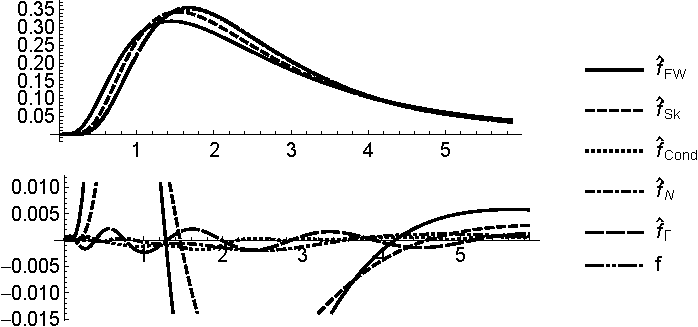
\includegraphics[width=0.8\textwidth]{d1.pdf}

\vspace{4mm}

\begin{tabular}{c|c|c|c|c|c|}
\cline{2-6}
                         & $\widehat{f}_{\mathrm{FW}}$  & $\widehat{f}_{\mathrm{Sk}}$ & $\widehat{f}_{\mathrm{Cond}}$ & $\widehat{f}_{\mathrm{N}}$  & $\widehat{f}_{\,\Gamma}$ \\ \hline
\multicolumn{1}{|c|}{$\Lp^2$} & $8.01 \stimes 10^{-2}$ & $4.00 \stimes 10^{-2}$ & $1.56 \stimes 10^{-3}$ & $1.94 \stimes 10^{-3}$ & $2.28 \stimes 10^{-3}$ \\  \hline
\end{tabular}
\caption*{Test 1: $\bfmu = (0, 0)$, $\diag(\bfSigma) = (0.5, 1)$, $\rho = -0.2$. Reference distributions used are $\NormDist(0.88,0.71^2)$ and $\GammaDist(2.43,0.51)$ with $K =$ 32, 16 resp.}
\end{figure}


\begin{figure}[H]
\centering
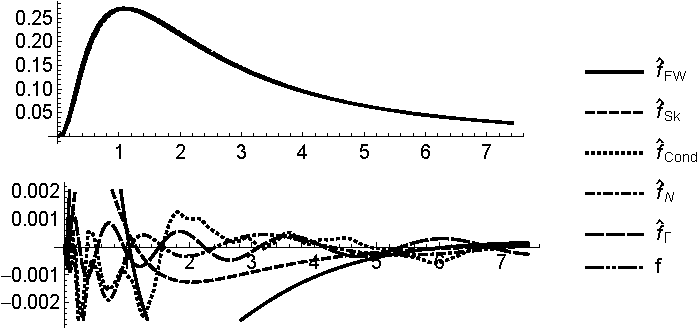
\includegraphics[width=0.8\textwidth]{d2.pdf}

\vspace{4mm}

\begin{tabular}{c|c|c|c|c|c|}
\cline{2-6}
                         & $\widehat{f}_{\mathrm{FW}}$  & $\widehat{f}_{\mathrm{Sk}}$ & $\widehat{f}_{\mathrm{Cond}}$ & $\widehat{f}_{\mathrm{N}}$  & $\widehat{f}_{\,\Gamma}$ \\ \hline
\multicolumn{1}{|c|}{$\Lp^2$} & $1.02 \stimes 10^{-2}$ & $3.49 \stimes 10^{-3}$ & $1.78 \stimes 10^{-3}$ & $7.86 \stimes 10^{-4}$ & $7.24 \stimes 10^{-4}$ \\ \hline
\end{tabular}
\caption*{Test 2: $\bfmu = (-0.5, 0.5)$, $\diag(\bfSigma)= (1,1)$, $\rho = 0.5$. Reference distributions used are $\NormDist(0.91,0.90^2)$ and $\GammaDist(2.35,0.51)$ with $K =$ 32, 16 resp.}
\end{figure}

\begin{figure}[H]
\centering
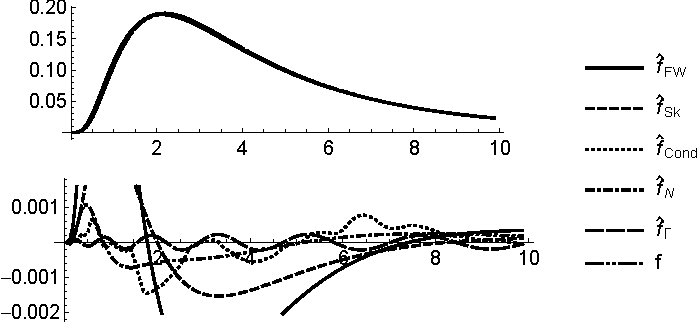
\includegraphics[width=0.8\textwidth]{d3.pdf}

\vspace{4mm}

\begin{tabular}{c|c|c|c|c|c|}
\cline{2-6}
                         & $\widehat{f}_{\mathrm{FW}}$  & $\widehat{f}_{\mathrm{Sk}}$ & $\widehat{f}_{\mathrm{Cond}}$ & $\widehat{f}_{\mathrm{N}}$  & $\widehat{f}_{\,\Gamma}$ \\ \hline
\multicolumn{1}{|c|}{$\Lp^2$} & $9.48 \stimes 10^{-3}$ & $3.71 \stimes 10^{-3}$ & $1.60 \stimes 10^{-3}$ & $1.18 \stimes 10^{-3}$ & $3.53 \stimes 10^{-4}$ \\ \hline
\end{tabular}
\caption*{Test 3: $n=3$, $\mu_i = 0$, $\Sigma_{ii} = 1$, $\rho = 0.25$. Reference distributions used are $\NormDist(1.32,0.74^2)$ and $\GammaDist(3,0.57)$ with $K =$ 7, 25 resp.}
\end{figure}


\begin{figure}[H]
\centering
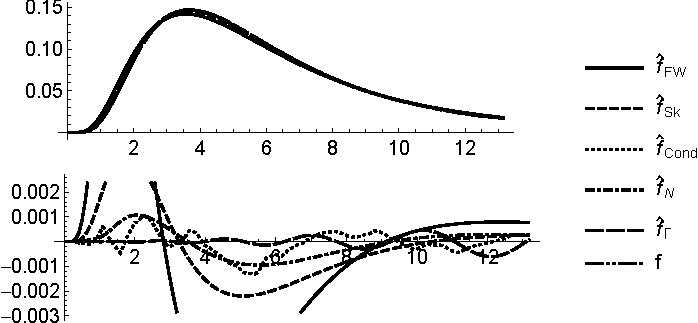
\includegraphics[width=0.8\textwidth]{d4.pdf}

\vspace{4mm}

\begin{tabular}{c|c|c|c|c|c|}
\cline{2-6}
                         & $\widehat{f}_{\mathrm{FW}}$  & $\widehat{f}_{\mathrm{Sk}}$ & $\widehat{f}_{\mathrm{Cond}}$ & $\widehat{f}_{\mathrm{N}}$  & $\widehat{f}_{\,\Gamma}$ \\ \hline
\multicolumn{1}{|c|}{$\Lp^2$} & $1.82 \stimes 10^{-2}$ & $6.60 \stimes 10^{-3}$ & $1.90 \stimes 10^{-3}$ & $1.80 \stimes 10^{-3}$ & $1.77 \stimes 10^{-4}$ \\ \hline
\end{tabular}
\caption*{Test 4: $n=4$, $\mu_i = 0$, $\Sigma_{ii}=1$, $\rho = 0.1$. Reference distributions used are $\NormDist(1.32,0.74^2)$ and $\GammaDist(3.37,0.51)$ with $K =$ 18, 18 resp.}
\end{figure}

The following test case shows the density approximations for a large $n$.

\begin{figure}[H]
\centering
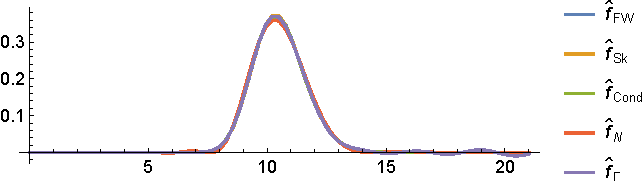
\includegraphics[width=0.8\textwidth]{d5.pdf}
\caption*{Test 5: Sum of 10 iid $\LNDist(0,0.1)$ random variables. Reference distributions used are $\NormDist(2.35,0.23^2)$ and $\GammaDist(12.61,0.25)$ with $K =$ 18, 35 resp.}
\end{figure}


Finally, we fit $\widehat{f}_{\mathrm{N}}$ and $\widehat{f}_{\,\Gamma}$ to simulated data ($10^5$ replications) for the sum of lognormals with a non-Gaussian dependence structure. Specifically, we take the sum of $n = 3$ standard lognormal random variables with a \emph{Clayton copula}, $\ClaytonCop(\theta)$, defined by its distribution function
\[
C^{\mathrm{Cl}}_\theta(u_1, \dots, u_n) = \Bigl( 1 - n + \sum_{i=1}^n u_i^{-\theta} \Bigr)^{-1/\theta}, \qquad \text{ for } \theta > 0 \,.
\]
The Kendall's tau correlation of the $C^{\mathrm{Cl}}_\theta$ copula is $\tau = \theta / (\theta + 2)$ \cite{mcneil2015quantitative}.

\begin{figure}
\centering
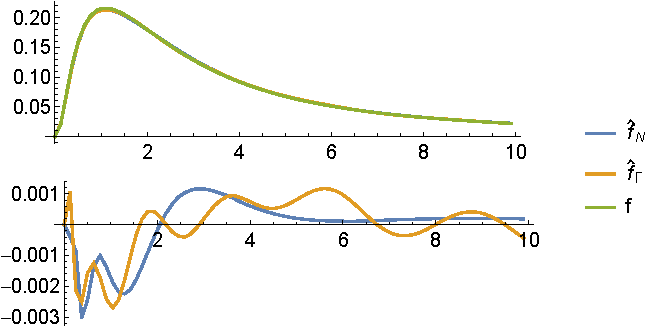
\includegraphics[width=0.8\textwidth]{copula.pdf}
\caption*{Test 6: Sum of 3 $\LNDist(0,1)$ random variables with $\ClaytonCop(10)$ copula (i.e., $\tau = \frac56$). Reference distributions used are $\NormDist(1.46,0.71^2)$ and $\GammaDist(8.78,0.25)$ with $K = 40$. The $\Lp^2$ errors of $\widehat{f}_{\mathrm{N}}$ and $\widehat{f}_{\,\Gamma}$ are $2.45 \times 10^{-3}$ and $2.04 \times 10^{-3}$ respectively.}
\end{figure}


Our overall conclusion of the numerical examples is that no single method can
be considered as universally superior. Of the methods in the literature,
the log skew normal approximations is generally better than Fenton-Wilkinson,
which is unsurprising given it is an extension introducing one more parameter.
The estimators, $\widehat{f}_{\mathrm{N}}$ and $\widehat{f}_{\,\Gamma}$, based on orthogonal polynomial approximation techniques, are very flexible. They also display at least as good and sometimes better pdf estimates over the interval $(0, \Exp[S])$ and their periodic error indicates that they would supply even more accurate cdf estimates. One should note, however, that their
performance relies on the tuning of parameters and that somewhat
greater effort is involved in their computation (though this is mitigated through the availability
of the software in \cite{OrthogoCode}).

An interesting feature of $\widehat{f}_{\mathrm{N}}$ and $\widehat{f}_{\,\Gamma}$ is that
the Clayton copula example indicates some robustness to the dependence structure used.
In view of the current interest in financial applications of non-Gaussian dependence this
seems a promising line for future research.

\begin{subappendices}
\section{Proof of \prop{LogNormalOrthogonalPolynomialProposition}} \label{app:lognormal_poly}
\begin{proof}
The polynomials which are orthogonal with respect to the lognormal distribution will be derived using the general formula \eqref{ortho_poly_gen_form}.
The moments of the $\LNDist(\mu, \sigma^2)$ distribution are given by $m_{n}=p^{n}q^{n^{2}}$, where $p=\e^{\mu}$ and $q=\e^{\frac{\sigma^{2}}{2}}$. Consider
\begin{equation}\label{eq:Dn1}
\bfH_n=\begin{pmatrix}
1&pq&\cdots&p^{n}q^{n^{2}} \\
pq&p^{2}q^{4}&&p^{n+1}q^{(n+1)^{2}}\\
\vdots&\vdots&&\vdots\\
p^{n-1}q^{(n-1)^{2}}&p^{n}q^{n^{2}}&\cdots&p^{2n-1}q^{(2n-1)^{2}}\\
p^{n}q^{n^{2}}&p^{n+1}q^{(n+1)^{2}}&\cdots&p^{2n}q^{(2n)^{2}}
\end{pmatrix}
\,, \quad n \in \NL\,,
\end{equation}
and denote by $R_{k}$ the $k$-th row and by $C_{\ell}$ the $\ell$-th column. Apply the elementary operations $R_{k+1}\rightarrow p^{-k}q^{-k^{2}}R_{k+1}$, and $C_{\ell+1}\rightarrow p^{-\ell}q^{-\ell^{2}}C_{\ell+1}$ for $k,\ell=0,\ldots,n$ to get
\begin{equation} \label{vand}
\bfA_n = \begin{pmatrix}
1 & \alpha_0 & \cdots & \alpha_0^n \\
1 & \alpha_1 & \cdots & \alpha_1^n \\
\vdots&\vdots&\vdots\\
1 & \alpha_{n-1} & \cdots & \alpha_{n-1}^n\\
1 & \alpha_n     & \cdots & \alpha_n^n
\end{pmatrix}
\,, \quad n \in \NL\,
\end{equation}
where $\alpha_i=q^{2i}$. As $\bfA_n$ is a Vandermonde matrix, $\det(\bfA_n) = \prod_{i=0}^{n} \prod_{j=i+1}^{n} (\alpha_j - \alpha_i)$, and
\begin{align}
\det(\bfH_n)
&= p^{n(n+1)} q^{\frac{n(n+1)(2n+1)}{3}} \det(\bfA_n) \label{detA_detH} \\
&= p^{n(n+1)} q^{\frac{n(n+1)(2n+1)}{3}}
\prod_{i=1}^{n} (-1)^i q^{2(n-i)i} [q^2; q^2]_i \,. \label{det_H}
\end{align}
Next, expand $\det(\tilde{\bfH}_n(x))$ with respect to the last row to get
\begin{equation}\label{eq:PolynomialExpression1}
p_{n}(x)=\frac{1}{\sqrt{\det(\bfH_{n-1})\det(\bfH_n)}}\sum_{k=0}^{n}(-1)^{n+k} \det(\bfC_{n,k}) x^{k},
\end{equation}
where $\bfC_{n,k}$ is $k$-th co-factor of $\bfH_n$ (i.e., $\bfH_n$ with the last row and the $(k+1)$-th column removed). Perform the same elementary operations as before on $\bfC_{n,k}$ to get
\begin{equation} \label{cofactor_det}
\det(\bfC_{n,k})=p^{n^{2}-k}q^{\frac{2n^{3}+n}{3}-k^{2}} \det( \bfA_{n,k} )
\end{equation}
where
\[ \bfA_{n,k} = \begin{pmatrix}
1&\alpha_{0}&\cdots&\alpha_{0}^{k-1}&\alpha_{0}^{k+1}&\cdots&\alpha_{0}^{n} \\
1&\alpha_{1}&\cdots&\alpha_{1}^{k-1}&\alpha_{1}^{k+1}&\cdots&\alpha_{1}^{n}  \\
\vdots&\vdots& &\vdots&\vdots&&\vdots\\
1&\alpha_{n-1}&\cdots&\cdots&\cdots&\cdots&\alpha_{n-1}^{n}
\end{pmatrix}  \,. \]

Using the definition of \emph{Schur polynomials}, it is clear that
\[ \det(\bfA_{n,k})  = s_{\lambda(k)}(\alpha_0,\dots,\alpha_{n-1}) \det(\bfA_{n-1}) \]
where $\lambda(k) = (\bfone_{n-k}, \bfzero_{k})$. With these $\lambda(k)$, the Schur polynomials simplify to the \emph{elementary symmetric polynomials}, so
\begin{equation} \label{vand_cofactor_det}
\det(\bfA_{n,k}) = e_{n-k}(\alpha_0,\dots,\alpha_{n-1}) \det(\bfA_{n-1}) \,.
\end{equation}
Combining \eqref{cofactor_det}, \eqref{vand_cofactor_det}, and \eqref{detA_detH} yields
\begin{align*}
\det(\bfC_{n,k})
&= p^{n^{2}-k}q^{\frac{2n^{3}+n}{3}-k^{2}} e_{n-k}(\alpha_0,\dots,\alpha_{n-1}) \det(\bfA_{n-1}) \\
&=  p^{n^{2}-k}q^{\frac{2n^{3}+n}{3}-k^{2}} e_{n-k}(\alpha_0,\dots,\alpha_{n-1}) p^{-n^2+n} q^{-\frac{(n-1)n(2n-1)}{3}} \det(\bfH_{n-1}) \\
&= p^{n-k} q^{n^2-k^2} e_{n-k}(\alpha_0,\dots,\alpha_{n-1}) \det(\bfH_{n-1}) \,.
\end{align*}
So, substituting this into the \eqref{eq:PolynomialExpression1} gives
\begin{align*}
p_{n}(x)
&=\frac{1}{\sqrt{\det(\bfH_{n-1})\det(\bfH_n)}}\sum_{k=0}^{n}(-1)^{n+k} p^{n-k} q^{n^2-k^2} e_{n-k}(\alpha_0,\dots,\alpha_{n-1}) \det(\bfH_{n-1}) x^{k} \\
&=  \sqrt{ \frac{ \det(\bfH_{n-1}) }{ \det(\bfH_n) } } p^{n} q^{n^2} \sum_{k=0}^{n}(-1)^{n+k} p^{-k} q^{-k^2} e_{n-k}(\alpha_0,\dots,\alpha_{n-1})  x^{k} \,.
\end{align*}
The constant $\det(\bfH_{n-1}) / \det(\bfH_n)$ can be handled using \eqref{det_H}
\begin{align*}
\frac{\det(\bfH_{n-1})}{\det(\bfH_n)}
&= p^{-2n} q^{-2n^2} \frac{ q^{-n(n-1)} }{ (-1)^n [q^2; q^2]_n  } =  \frac{ p^{-2n} q^{-3n^2+n} }{\abs{ [q^2; q^2]_n } } \,.
\end{align*}
Finally, simplify this constant using $q^{n + n^2}/ \abs{ [q^2; q^2]_n } = 1/[q^{-2}; q^{-2}]_n$ to get \eqref{eq:OrthonormalPolynomialLogNormalExpression}.
\end{proof}

\section{Computing the coefficients of the expansion $\{a_{k}\}_{k\in\NZ}$
in the gamma case} \label{app:proof}

We extend here the above techniques to construct an approximation
for $\Laplace_i(\theta)$. We note that $\Laplace_i(\theta) \propto \int_{\RL^n} \exp\{ -h_{\theta,i}(\bfx) \} \dd \bfx $ where
\[ h_{\theta,i}(\bfx) = - i \ln(\bfone^\tr \ve^{\bfmu + \bfx}) + \theta \bfone^\tr \ve^{\bfmu + \bfx} + \frac12 \bfx^\tr \bfSigma^{-1} \bfx \,, \quad i \in \NZ \,. \]
This uses the notation of the previous chapter, where for example, $\ve^{\bfx} = (\e^{x_1}, \dots, \e^{x_n})^\top$. Next, define $\bfx^*$ as the minimiser of $h_{\theta,i}$ (calculated numerically), and consider a second order Taylor expansion of $h_{\theta,i}$ about $\bfx^*$. Denote $\widetilde{\Laplace}_i(\theta)$ as the approximation of $\Laplace_i(\theta)$ in which $h_{\theta,i}$ is replaced by this Taylor expansion. Simplifying yields
\begin{equation} \label{firstTerm}
	\widetilde{\Laplace}_i(\theta) = \frac{ \exp\{-h_{\theta,i}(\bfx^*)\} }{ \sqrt{ \abs{\det(\bfSigma \bfH)} }}
\end{equation}
where $\bfH$, the Hessian of $h_{\theta,i}$ evaluated at $\bfx^*$, is
\[ \bfH = i\frac{\ve^{\bfmu + \bfx^*} (\ve^{\bfmu + \bfx^*})^\tr}{(\bfone^\tr \ve^{\bfmu + \bfx^*})^2} + \bfSigma^{-1} - \diag(\bfSigma^{-1} \bfx^*) \,. \]

As $\theta \to \infty$ we have $\widetilde{\Laplace}_i(\theta) \to \Laplace_i(\theta)$. We rewrite $\Laplace_i(\theta) = \widetilde{\Laplace}_i(\theta) I_i(\theta)$ and estimate $I_i(\theta)$ as follows.

\begin{proposition} \label{prop:laplace_derivatives}
The moments of the $\SLNDist_\theta(\bfmu, \bfSigma)$ distribution, denoted $\Laplace_i(\theta)$, can be written as $\Laplace_i(\theta) = \widetilde{\Laplace}_i(\theta) I_i(\theta)$, where $\widetilde{\Laplace}_i(\theta)$ is in \eqref{firstTerm}, and
\begin{align*}
	I_i(\theta) &= \sqrt{\abs{\det(\bfSigma \bfH)}} \, v(\bfzero)^{-1} \, \Exp[v(\bfSigma^{\frac12} \bfZ)]
\end{align*}
for $\bfZ \sim \NormDist(\bfzero, \bfeye)$, and
\[ v(\bfz) = \exp\{ i \ln(\bfone^\tr \ve^{\bfmu + \bfx^* + \bfz}) - \theta \bfone^\tr \ve^{\bfmu + \bfx^* + \bfz} - (\bfx^*)^\tr \bfSigma^{-1} \bfz \} \,. \]
\end{proposition}
\begin{proof}
Substitute $\bfx = \bfx^* + \bfH^{-\frac12} \bfy$ into $\Laplace_i(\theta)$, then multiply by $\exp\{ \pm \text{ some constants}\}$:
\begin{align*}
	\Laplace_i(\theta) &= \int_{\RL^n} \frac{ (2\pi)^{-\frac{n}{2}} }{\sqrt{\abs{\det(\bfSigma)}}} \exp\{ i \log(\bfone^\tr \ve^{\bfmu + \bfx}) - \theta \bfone^\tr \ve^{\bfmu + \bfx} - \frac12 \bfx^\tr \bfSigma^{-1} \bfx \}  \dd \bfx \\
	&= \widetilde{\Laplace}_i(\theta) \exp\{ -i \log(\bfone^\tr \ve^{\bfmu + \bfx^*}) + \theta \bfone^\tr \ve^{\bfmu + \bfx^*} \} \\
	&\qquad \times \int_{\RL^n} (2\pi)^{-\frac{n}{2}} \exp\{ i \log(\bfone^\tr \ve^{\bfmu + \bfx^* + \bfH^{-\frac12} \bfy}) - \theta \bfone^\tr \ve^{\bfmu + \bfx^* + \bfH^{-\frac12} \bfy} \\
	&\qquad\qquad -(\bfx^*)^\tr \bfSigma^{-1} \bfH^{-\frac12} \bfy - \frac12 \bfy^\tr (\bfSigma \bfH)^{-1} \bfy \}  \dd \bfy \,.
\end{align*}
That is, $\Laplace_i(\theta) = \widetilde{\Laplace}_i(\theta) I_i(\theta)$. In $I_i(\theta)$, take the change of variable $\bfy = (\bfSigma\bfH)^{\frac12} \bfz$, and the result follows.
\end{proof}


\begin{remark}
The form of $I_i(\theta)$ naturally suggests evaluation using \emph{Gauss--Hermite} quadrature:
\begin{equation} \label{eq:gauss-hermite-quad}
	\widehat{\Laplace}_i(\theta) = \frac{\exp\{-h_{\theta,i}(\bfx^*)\}}{v(\bfzero) \,\pi^{\,n/2}} \sum_{i_1=1}^H \cdots \sum_{i_n=1}^H v(\bfSigma^{\frac12} \bfz)  \prod_{j=1}^n w_{i_j}
\end{equation}
where $\bfz = (z_{i_1}, \dots, z_{i_n})^\top$, the set of weights and nodes $\{(w_i, z_i) : 1 \le i \le H\}$ is specified by the Gauss--Hermite quadrature algorithm, and $H \ge 1$ is the order of the approximation. This approximation is accurate, especially so when the $i$ in $\Laplace_i$ becomes large. Even for $\Laplace$ ($= \Laplace_0$) this method appears to outperform the quasi-Monte Carlo scheme outlined in Chapter~\ref{chp:Laplace}. \remQED
\end{remark}



Thus, with $\widehat{\Laplace}_i(\theta)$ given in \eqref{eq:gauss-hermite-quad}, we can now estimate the coefficients. The three methods correspond to
\begin{enumerate}
\item $\widehat{a}_k = R^{-1} \sum_{r=1}^R p_k(S_r)$, for $S_1$, \dots, $S_R \iidDist f_\theta(x)$,
\item $\widehat{a}_k = \sum_{j=0}^k q_{kj} \, \widehat{\Exp[S_\theta^j]} = q_{k0} + (R \, \widehat{\Laplace}(\theta))^{-1} \sum_{j=1}^k q_{kj} \sum_{r=1}^R S_r^j \e^{-\theta S_r}$, from \eqref{eq:expand_coeffs}, where $S_1$, \dots, $S_R \iidDist f(x)$,
\item $\widehat{a}_k = q_{k0} + \widehat{\Laplace}(\theta)^{-1} \sum_{j=1}^k q_{kj} \, \widehat{\Laplace}_j(\theta)$.
\end{enumerate}
In the numerical illustrations, we switched between using methods (2) and (3) for large and small $n$ respectively. Algorithms for efficient simulation from $f_\theta$ is work in progress.


\end{subappendices}